\section{Appendix: Protocol Descriptions}

Data structures in the ABNF\footnote{\url{https://tools.ietf.org/html/rfc5234}} format:

\begin{lstlisting}[language=abnf]
token = tokenId, tokenClass, tokenValue, mint, transition*, token-state

mint = mintProofs, mintRequest, mintSalt, genesis
mintProofs = path*
mintRequest = destPointer
genesis = challenge

path = unicityProof, payload, authenticator   ; leaf <\~=> unicityProof

payload = hash       ; payload <- h(h(source.challenge) || destPointer || salt)
authenticator = state-hash, pubkey, signature   ; owner's signature

transition = tokenId, source, input, destination   ; token history record, with proofs
input = path*, destPointer, salt  ; sender's proof of the ownership and Unicity (single-spend) proof
source      = challenge   ; owner id
destination = challenge   ; newowner id

token-state = challenge   ; owner id

destPointer = hash  ; destPointer <- h(tokenClass || pubkey || nonce)
                    ; Destination pointer: the pointer refering the hidden expected token's destination state. recipient --> sender
                    ; masked NewOwner

challenge = tokenClass, tokenId, pubkey, nonce    ; a challenge for the respective private key to 'solve'
         ;  like 'address'

; ----------- token+transaction are delivered to the new owner.
transaction = tokenId, source, input, destPointer

; -----------
tokenId = tokenClass = hash
tokenValue = DIGIT+
salt = mintSalt = 64(HEXDIG)
nonce = 64(HEXDIG)
state-hash = hash
pubkey = 130(HEXDIG)
signature = 144(HEXDIG)
hash = 64(HEXDIG)
DIGIT = %x30-39
HEXDIG = %x30-39 / %x41-46 / %x61-66
\end{lstlisting}




\begin{figure}[!htbp]
        \begin{center}
        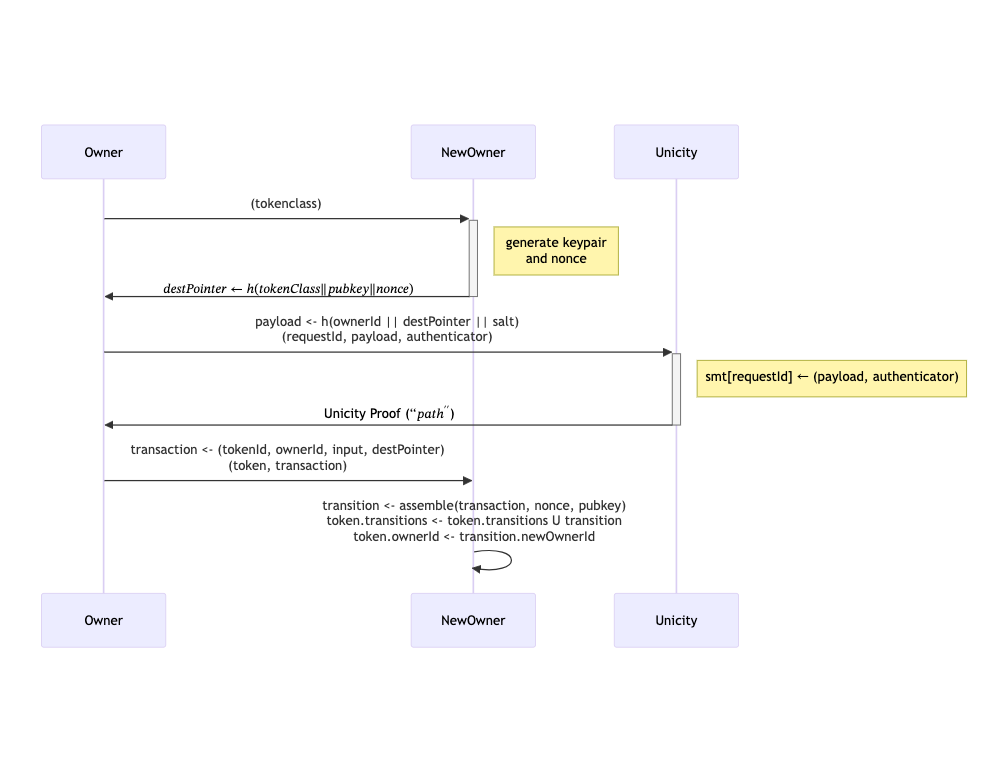
\includegraphics[width=\textwidth]{unicity-tx}
        \caption{Data flow of a Transaction}\label{fig:tx}
        \end{center}
\end{figure}
% https://mermaid.live/edit#pako:eNp9U8Fu2zAM_RVBMFAbc7q7UeSyXXJYW2DoZdOAKhZjC7UlV6JRBIn_fZSsOG47zBdLJB8f-SieeG0V8Ip7eB3B1PBdy8bJXhhG38ObAbfZbr_cw1s8VyxH-0JxnfS-mIPuLQJzummR2QO7RjZAP0m-FzgOUru7vfu6lUYxY4knYVM0cWwSLMuE6CW2_nBS4PHRaoPgJiZEA-hZmy_uWMm3UEnwntniGMY9cX4wRtapoPTvW3syutZ4rNggj52Vit1tiMQG906x85mtqghXLzssYi-5C5p53KnyAi6ZHLEFg7qWaN0_FVoIfY-_lxR_YuOhxSxj-X_TpQQrzZKFPTpLBPlKwufngQ43N1OWFe8bvw4KnTRe1qitCc3PEw5NJRFKps0wYrlWIikQQ8t1huLTYD8Q6QsPzQ36fQf5Cl3Oj4P0jCOcWSLJ7RXsA_qz8WmVf4W7TDJgFv-tSUXtlDC85D24XmpFe3AK9QtOqvcgeEVHBQc5dii4MBOF0kTsz6OpeYVuhJI7OzYtrw6y83QbB0VPPi3RYh2k-WXt9Q5K0zh_zJsXF3D6C_AtPcg



\subsection{Token Transfer (with blinding)}

\begin{lstlisting}
     0. owner has a token:
        token = tokenId, tokenClass, tokenValue, mint, transition*, token-state

     1. new owner:
        - generates a fresh keypair and a blinding factor (nonce)
          (newOwnerPk, newOwnerSk) <- Gen(\lambda)
          nonce <$ {0,1}^256
        - calculates a pointer, sends to owner. Pointer ~ blinded recipient
          destPointer <- h(tokenClass || newOwnerPk || nonce)
        - sends it to owner

     2. owner:
        - generate random salt
          salt <$ {0,1}^256
        - sends a request to Unicity Service:
          blindedOwnerId <- h(token-state)      ; token.state = transition.source = transaction.source
          payload <- h(blindedOwnerId || destPointer || salt)
          ; Note that blindedOwnerId is also token identifier because the owner id is unique one-time id; and called "token state" as ownership is the only immutable field; more consistent naming is needed
          RequestId <- h(ownerPk || blindedOwnerId)
          authenticator <- (blindedOwnerId, ownerPk, Sig_ownerSk(payload))
          Submit_request(RequestId, payload, authenticator)
        - Obtain Unicity Proof
          (RequestId, (payload, authenticator), path) <- Get_proof(RequestId)
        - Create tx:
          input <- (path, destPointer, salt)  ; where path is unicity proof, salt is sender's blinding factor
          transaction <- (tokenId, token.state, input, destPointer)   ; state ~ current owner

     3. send tx to new owner:
          send (token, transaction)

     4. new owner receives (token, transaction) and finalizes the token:
        - recall the keypair and nonce generated during step 1
        - convert transaction to transition, append transition to transition history, and set new owner:
          destination <- (token.tokenClass, token.tokenId, pubkey, nonce)
          transition <- (transaction.tokenId, transaction.source, transaction.input, destination)
              token.transitions <- token.transitions U transition
              token.state <- transition.destination   ; the owner field

\end{lstlisting}

\subsection{Unicity Service}

Provides two services: 1) set a key-value in key-value store:

\begin{lstlisting}
Set a key-value pair (if not set)
input: (RequestId, payload, authenticator)

1. If the key RequestId is set then return error
2. Validate the request:
2.1 check if the sender is in possession of private key the OwnerAddress and RequestId are derived from
2.1.1 verify the signature on whatever:
        Ver_{authenticator.ownerPk}(payload) = 1
2.1.2 verify if RequestId is derived correctly:
        RequestId = h(authenticator.ownerPk || authenticator.blindedOwnerId)
2.1.3 verify if TransitionCommitment is fresh or related to this request
        not needed, as there is assumption that (ownerPk, ownerSk) is not reused.
3 Write the key
smt[RequestId] <- (payload, authenticator)
\end{lstlisting}

... and 2) return a key-value+proof:

\begin{lstlisting}
Return a key-value pair (if set)
input: (RequestId)
output: (RequestId, (payload, authenticator), unicityProof)

1. return error if smt[RequestId] is not set
2. return (requestId, smt[RequestId], unicityProof)
   where unicityProof is hash chain and finality gadget's signature
\end{lstlisting}



\subsection{Token Validation}

\begin{lstlisting}
Token validation:
input: token
output: ok or not

1. validate "path"s , that is, signature + Unicity Proof pairs.
     Ver_{token.transition[i].input.path[j].authenticator.ownerPk}(token.transition[i].input.path[j].payload,
         token.transition[i].input.path[j].authenticator.signature) = 1
     \forall p <- token.transition[i].input.path[j]:
        Ver_{p.authenticator.ownerPk}(p.payload, p.authenticator.signature) = 1
   Unicity Cert:
     \forall p <- token.transition[i].input.path[j]:
       requestId <- Ver_{UTB}((p.payload, p.authenticator), tp.unicityCert)
       requestId = h(p.authenticator.ownerPk || p.authenticator.blindedOwnerId)
2. consistency
     \forall t <- token.transition[i]:
       t.input.path[j].payload = h(source.blindedOwnerId || t.input.destPointer || t.input.salt)
     token.token-state.challenge = token.transition[-1].destination.challenge

     token.transition[i].destination.challenge = token.transition[i+1].source.challenge


\end{lstlisting}
